
\newpage

\section{Model}



Om een goed verhaal op te stellen, moet vooraf aan enkele voorwaarden
worden voldaan. De eerste voorwaarde is de geschiktheid van het
afstudeerproject. Als een afstudeerproject niet tot keuzes leidt, kan
men zich afvragen of dat wel een echte afstudeeropdracht is. Een
afstudeerproject zonder onderzoeksaspecten is ook verdacht. Daarnaast
moet een afstudeerproject passen in het profiel van een opleiding om
beoordeelbaar te zijn. De andere voorwaarde voor goed een verhaal is
de registratie van werkzaamheden tijdens het a


	%%%%%%%%%%%%%%%%%%%%%%%%%%%%%%%%%%%%%%%%%%%%%%%%%%%%%%%%%%%%%%


\begin{center}
	\figuur{width=\columnwidth}{plaatjes/stroomschema\_sluispassage.png}{PNGR}{Variabele breedte (png)}
\end{center}
%%%%%%%%%%%%%%%%%%%%%%%%%%%%%%%%%%%%%%%%%%%%%%%%%%%%%%%%%%%%%%
\subsection{scenario en use case}



Om een goed verhaal op te stellen, moet vooraf aan enkele voorwaarden
worden voldaan. De eerste voorwaarde is de geschiktheid van het
afstudeerproject. Als een afstudeerproject niet tot keuzes leidt, kan
men zich afvragen of dat wel een echte afstudeeropdracht is. Een
afstudeerproject zonder onderzoeksaspecten is ook verdacht. Daarnaast
moet een afstudeerproject passen in het profiel van een opleiding om
beoordeelbaar te zijn. De andere voorwaarde voor goed een verhaal is
de registratie van werkzaamheden tijdens het a

\begin{usecase}
	\addheading{Actor}{System user} 
	\addrow{Precondition}{The system, shows, in the form part of an object type, the number   indication.}
	\addrow{Postcondition}{A disconnected number indicating the type of `other constructed object'.}
	\addmulrow{Main path (M)}{\item User selects \ldots
		\item System demands \ldots}
\end{usecase}
\subsection{De Kripke structuur}

Om een goed verhaal op te stellen, moet vooraf aan enkele voorwaarden
worden voldaan. De eerste voorwaarde is de geschiktheid van het
afstudeerproject. Als een afstudeerproject niet tot keuzes leidt, kan
men zich afvragen of dat wel een echte afstudeeropdracht is. Een
afstudeerproject zonder onderzoeksaspecten is ook verdacht. Daarnaast
moet een afstudeerproject passen in het profiel van een opleiding om
beoordeelbaar te zijn. De andere voorwaarde voor goed een verhaal is
de registratie van werkzaamheden tijdens het a

\subsection{title}

 
\subsection{Soorten modellen}

Om een goed verhaal op te stellen, moet vooraf aan enkele voorwaarden
worden voldaan. De eerste voorwaarde is de geschiktheid van het
afstudeerproject. Als een afstudeerproject niet tot keuzes leidt, kan
men zich afvragen of dat wel een echte afstudeeropdracht is. Een
afstudeerproject zonder onderzoeksaspecten is ook verdacht. Daarnaast
moet een afstudeerproject passen in het profiel van een opleiding om
beoordeelbaar te zijn. De andere voorwaarde voor goed een verhaal is
de registratie van werkzaamheden tijdens het a
\subsection{Tijd}

Om een goed verhaal op te stellen, moet vooraf aan enkele voorwaarden
worden voldaan. De eerste voorwaarde is de geschiktheid van het
afstudeerproject. Als een afstudeerproject niet tot keuzes leidt, kan
men zich afvragen of dat wel een echte afstudeeropdracht is. Een
afstudeerproject zonder onderzoeksaspecten is ook verdacht. Daarnaast
moet een afstudeerproject passen in het profiel van een opleiding om
beoordeelbaar te zijn. De andere voorwaarde voor goed een verhaal is
de registratie van werkzaamheden tijdens het a
\subsection{Guards en invarianten}

Om een goed verhaal op te stellen, moet vooraf aan enkele voorwaarden
worden voldaan. De eerste voorwaarde is de geschiktheid van het
afstudeerproject. Als een afstudeerproject niet tot keuzes leidt, kan
men zich afvragen of dat wel een echte afstudeeropdracht is. Een
afstudeerproject zonder onderzoeksaspecten is ook verdacht. Daarnaast
moet een afstudeerproject passen in het profiel van een opleiding om
beoordeelbaar te zijn. De andere voorwaarde voor goed een verhaal is
de registratie van werkzaamheden tijdens het a
\subsection{Deadlock}

Om een goed verhaal op te stellen, moet vooraf aan enkele voorwaarden
worden voldaan. De eerste voorwaarde is de geschiktheid van het
afstudeerproject. Als een afstudeerproject niet tot keuzes leidt, kan
men zich afvragen of dat wel een echte afstudeeropdracht is. Een
afstudeerproject zonder onderzoeksaspecten is ook verdacht. Daarnaast
moet een afstudeerproject passen in het profiel van een opleiding om
beoordeelbaar te zijn. De andere voorwaarde voor goed een verhaal is
de registratie van werkzaamheden tijdens het a
\subsection{Zeno gedrag}

Om een goed verhaal op te stellen, moet vooraf aan enkele voorwaarden
worden voldaan. De eerste voorwaarde is de geschiktheid van het
afstudeerproject. Als een afstudeerproject niet tot keuzes leidt, kan
men zich afvragen of dat wel een echte afstudeeropdracht is. Een
afstudeerproject zonder onderzoeksaspecten is ook verdacht. Daarnaast
moet een afstudeerproject passen in het profiel van een opleiding om
beoordeelbaar te zijn. De andere voorwaarde voor goed een verhaal is
de registratie van werkzaamheden tijdens het a
\section{Logica}

Om een goed verhaal op te stellen, moet vooraf aan enkele voorwaarden
worden voldaan. De eerste voorwaarde is de geschiktheid van het
afstudeerproject. Als een afstudeerproject niet tot keuzes leidt, kan
men zich afvragen of dat wel een echte afstudeeropdracht is. Een
afstudeerproject zonder onderzoeksaspecten is ook verdacht. Daarnaast
moet een afstudeerproject passen in het profiel van een opleiding om
beoordeelbaar te zijn. De andere voorwaarde voor goed een verhaal is
de registratie van werkzaamheden tijdens het a




\subsubsection{Uppaal syncrhonisatie}




Templates automata are defined with a set of parameters that can be of any
type (e.g., int, chan). These parameters are substituted for a given argument
in the process declaration.
Constants are declared as const name value. Constants by definition cannot
be modified and must have an integer value.
Bounded integer variables are declared as int[min,max] name, where min
and max are the lower and upper bound, respectively. Guards, invariants, and
assignments may contain expressions ranging over bounded integer variables.
The bounds are checked upon verification and violating a bound leads to an
invalid state that is discarded (at run-time). If the bounds are omitted, the
default range of -32768 to 32768 is used.
Binary synchronisation channels are declared as chan c. An edge labelled
with c! synchronises with another labelled c?. A synchronisation pair is
chosen non-deterministically if several combinations are enabled.
Broadcast channels are declared as broadcast chan c. In a broadcast synchronisation
one sender c! can synchronise with an arbitrary number of
receivers c?. Any receiver than can synchronise in the current state must do
so. If there are no receivers, then the sender can still execute the c! action,
i.e. broadcast sending is never blocking.
Urgent synchronisation channels are decalred by prefixing the channel declaration
with the keyword urgent. Delays must not occur if a synchronisation
transition on an urgent channel is enabled. Edges using urgent channels for
synchronisation cannot have time constraints, i.e., no clock guards.
Urgent locations are semantically equivalent to adding an extra clock x, that
is reset on all incomming edges, and having an invariant x<=0 on the location.
Hence, time is not allowed to pass when the system is in an urgent location.
Committed locations are even more restrictive on the execution than urgent
locations. A state is committed if any of the locations in the state is committed.
A committed state cannot delay and the next transition must involve
an outgoing edge of at least one of the committed locations.
Arrays are allowed for clocks, channels, constants and integer variables. They
are defined by appending a size to the variable name, e.g. chan c[4]; clock
a[2]; int[3,5] u[7];.
Initialisers are used to initialise integer variables and arrays of integer variables.
For instance, int i := 2; or int i[3] := {1, 2, 3};.
 


\paragraaf{Werken met Uppaal}

Het is niet verplicht om met \LaTeX{} te werken. Men mag ook gebruik
maken van andere tekstverwerkers zoals \emph{MS-Word}, Wel is het
verplicht het afstudeerverslag \LaTeX{}-geformateerd in te leveren en
van de \LaTeX{}-template \verb!modelverslag.sty! gebruik te
maken.

De \LaTeX{}-template bevat enkele macro's voor het opstellen van een
hoofdstuk (\verb!\hoofdstuk!), een paragraaf (\verb!\paragraaf!), een
afbeelding (\verb!\figuur!). De overige \LaTeX{} macro's en omgevingen
blijven bruikbaar. Bijvoorbeeld de \verb!tabular!-omgeving om tabellen
te maken:

\begin{lstlisting}{language=[LaTeX]TeX}
	\begin{tabular}{formaat}
		... 
	\end{tabular}
\end{lstlisting}
 

\begin{center}
	\begin{tabular}{|l||r|}
		\hline
		\multicolumn{2}{|c|}{use case omschrijving}\\
		\hline
		Aanvaren     & \the\paperwidth\\
		Aanmelden      & \the\textwidth\\
		Wachten    & \the\columnwidth\\
		Deuren openen & \the\columnsep\\
		uitvaren  & \the\oddsidemargin\\
		invaren & \the\evensidemargin\\
		Deuren sluiten    & \the\paperheight\\
		Nivelleren     & \the\textheight\\
		Deuren openen & \the\columnsep\\
		uitvaren  & \the\oddsidemargin\\
	 
		\hline
	\end{tabular}
\end{center}

Een nadeel van tabellen dat ze vaak te groot zijn voor de
twocolumn-mode. Het zou mooi zijn als ze ingedrukt kunnen
worden. Bovendien is deze tabel niet-zwevend, hij wordt geplaatst
tussen de tekstdelen waar hij is ingevoerd. Dit kan bezwaarlijk zijn
bij pagina-overgangen. In dat geval kan je beter gebruikmaken van
zwevende tabellen (en figuren) die door \LaTeX{} zelf op een geschikte
plaats worden gezet. Wel moet aan een zwevende tabel een label en een
onderschrift gekoppeld worden om er naar te kunnen verwijzen. Voor een
zwevende horizontale tabel met label en onderschrift wordt in de
`template' de \verb!tabel!-omgeving aangeboden:\\

\begin{Aanpassen}
	\begin{verbatim}
		\begin{tabel}[afm]{formaat}{label}{onderschrift}
			...
		\end{tabel}
	\end{verbatim}
\end{Aanpassen}


De \verb!tabel!-omgeving plaatst `zwevende' tabellen in verslag- en
publicatie-mode. Het eerste argument is een optioneel \verb![afm]!
argument met de defaultwaarde \verb!\normalsize! voor de afmeting van
de karakters. De mogelijke waarden voor de afmeting zijn -- van groot
tot klein -- de volgende macro's: (\verb!\huge!, \verb!\LARGE!,
\verb!\Large!, \verb!\large!, \verb!\small!, \verb!\footnotesize!,
\verb!\scriptsize! en \verb!\tiny!).

Bovendien zijn de standaard \verb!tabular! kolomformaten
\verb!r,l,c,|,||,p{lengte}! uit de tabelomgeving uitgebreid met
kolomformaten \verb!\R, \C, \L!  voor variabele celinhoud zoals het
plaatsen van meerdere regels per cel.

Een verticale tabel is mogelijk met de omgeving (\verb!TABEL!)  met
dezelfde kolomformaten mogelijkheden.  In \LaTeX{} zijn de tabellen,
vooral in de \verb!twocolumn!-mode erg lastig. Bijvoorbeeld in de
tabellen~\ref{tab:vbt} en \ref{tab:vbx} zijn twee verschillende
uitwerkingen van de tabelomgevingen:

\begin{footnotesize}
	\begin{tabel}[\Large]{|r|l|}{vbt}{Vaste cellen, variabele breedte}
		\hline
		7C0 & hexadecimal \\
		3700 & octal \\ \cline{2-2}
		11111000000 & binary \\
		\hline \hline
		1984 & decimal \\
		\hline
	\end{tabel}
\end{footnotesize}

%Absolute breedte in mm, cm etc. (geschikt voor één mode):
%\begin{tabel}{|>\R p{2cm}|>\L p{4cm}|}{vbx}{OpenGL libraries}
%Relatieve breedte 20% en 65% van de kolombreedte (geschikt voor alle moden).
%Procentwaarden van 0 ... 99, voor 100% neem \columnwidth zelf.
\begin{tabel}{|>\R p{\Procent{20}}|>\L
		p{\Procent{65}}|}{vbx}{Variabele cellen, variabele breedte}
	\hline
	OpenGL core library & OpenGL32 voor MS-Windows en GL voor
	de meeste X-Window systemen\\
	\hline
	OpenGL Utility Library & GLU\\
	\hline
	Koppeling met het platform & GLX voor X-Window en WGL voor MS-Windows\\
	\hline 
	OpenGL Library Utility Toolkit & GLUT, bibliotheek voor
	het openen van windows, invoer van muis en toetsenbord, menus,
	event-driven in- en uitvoer\\
	\hline
\end{tabel}

Plaats afbeeldingen alleen in het hoofdverslag als ze de tekst
ondersteunen en de leesbaarheid niet verlagen.  In de tekst kan naar
afbeeldingen worden verwezen met de macro \verb!\ref{fig:label}!.

In \LaTeX{}\cite{lam1994} geschreven verslagen zijn op diverse manieren
afbeeldingen\cite{Oos1996} te plaatsen. Een van die manieren is gebruik te
maken van de macro \verb!\figuur! in de \verb!modelverslag!-package'.

`Vector graphics' figuren van het `pdf-', `eps-' en `svg-'
formaat\footnote{Een pdf-bestand kan zowel vector-graphics als
	bitmap-graphics bevatten.} met een ingewikkelde `bounding box' zijn
moeilijk op de juiste schaal te brengen. Vaak moet dat met uitproberen
bepaald worden. Het plaatsen van figuren met absolute afmetingen of
een vaste `scale' factor, kan leiden tot minder soepele oplossingen
zoals figuur~\ref{fig:PDFA}. Deze figuur heeft naast een rotatie
(\verb!angle=270!)  een vaste scale-factor (\verb!scale=0.45!) die
alleen geschikt is voor de `twocolumn-mode'.



\begin{center}
	\begin{tabular}{|>\C p{\Procent{80}}|}
		\hline
		~\\
		Use case\\
		~\\
		Tabellen, figuren en listingen in het hoofdverslag tot het
		noodzakelijke beperken.\\
		~\\
		\hline
	\end{tabular}
\end{center}




\begin{center}
	
	\figuur{width=\columnwidth}{plaatjes//2020/eerste oplevermoment/Deuren.png}{PNGR}{Variabele breedte (png)}
\end{center}



In plaats van \verb!scale=x! kan je beter de relatieve afmeting
\verb!width=\Procent{y}! gebruiken. De waarde $y$ wordt in de
verslag-mode met uitproberen gevonden, zie figuur~\ref{fig:PDFR}.

\begin{center}
	
	\figuur{width=\columnwidth}{plaatjes/2020/eerste oplevermoment/knop.png}{PNGR}{Variabele breedte (png)}
\end{center}


Het afmetingsprobleem is iets gemakkelijker op te lossen met `bitmap
graphics' van het `jpg-', `gif-' en `png-' formaat omdat de figuren al
van te voren geschaald kunnen worden als de `bounding box' bij het
inlezen bekend is. De breedte (\verb!width!) kan als percentage van de
kolombreedte (\verb!width=\Procent{0 ... 99}!) worden opgegeven zoals
dat bij figuur~\ref{fig:PNGR} gedaan is. Voor een 100\% waarde neemt
men \verb!width=\columnwidth! De afmeting wordt automatisch
aangepast aan de nieuwe kolombreedte.



\begin{center}
	\begin{tabular}{|>\C p{\Procent{80}}|}
		\hline
		~\\
		Use case\\
		~\\
		Wachten voor de sluis\\
		~\\
		\hline
	\end{tabular}
\end{center}

\begin{center}
	
	\figuur{width=\columnwidth}{plaatjes/2020/eerste oplevermoment/lamp.png}{PNGR}{Variabele breedte (png)}
\end{center}




\begin{center}
	\begin{tabular}{|>\C p{\Procent{80}}|}
		\hline
		~\\
		Use case\\
		~\\
	Sluis invaren\\
		~\\
		\hline
	\end{tabular}
\end{center}

\begin{center}
	
	\figuur{width=\columnwidth}{plaatjes/2020/eerste oplevermoment/Sensor.png}{PNGR}{Variabele breedte (png)}
\end{center}




\begin{center}
	\begin{tabular}{|>\C p{\Procent{80}}|}
		\hline
		~\\
		Use case\\
		~\\
		Sluis uitvaren\\
		~\\
		\hline
	\end{tabular}
\end{center}

\begin{center}
	
	\figuur{width=\columnwidth}{plaatjes/2020/eerste oplevermoment/Sluis.png}{PNGR}{Variabele breedte (png)}
\end{center}

\begin{center}
	
	\figuur{width=\columnwidth}{plaatjes/2020/eerste oplevermoment/ship.png}{PNGR}{Variabele breedte (png)}
\end{center}

\begin{center}
	
	\figuur{width=\columnwidth}{plaatjes/2020/eerste oplevermoment/Stoplicht.png}{PNGR}{Variabele breedte (png)}
\end{center}




\begin{center}
	\begin{tabular}{|>\C p{\Procent{80}}|}
		\hline
		~\\
		Use case\\
		~\\
		Meerdere niveaus\\
		~\\
		\hline
	\end{tabular}
\end{center}

De macro \verb!\PROCENT{0...99}! is nodig voor de macro's \verb!Tabel!
en \verb!Figuur!. Deze laatste twee macro's maken het mogelijk dat
tabellen en afbeeldingen in de twocolumn-mode passen met behoud van
hun originele afmeting en detaillering (zie
figuur \ref{fig:FIXED}). De parameters van deze macro's komen overeen
met de parameters van de macro's \verb!tabel! en \verb!figuur!.


\begin{center}
	
	\figuur{width=\columnwidth}{plaatjes/2020/eerste oplevermoment/ship.png}{PNGR}{Variabele breedte (png)}
\end{center}

\begin{center}
	
	\figuur{width=\columnwidth}{plaatjes/2020/eerste oplevermoment/Stoplicht.png}{PNGR}{Variabele breedte (png)}
\end{center}

In het algemeen heeft vector-graphics een betere kwaliteit van de
weergave dan bitmap-graphics.


\paragraaf{Bijzondere tekens en afbreekproblemen}

Bijzondere tekens zoals de á, à, ä, é, è, ë, ï, ü, ç \ldots worden
probleemloos door \LaTeX{} geaccepteerd als normale utf8
karakters. Voor de uitzonderingen bestaan macro's zoals het
euro-symbool \euro{} waarvoor de macro \verb!\euro! nodig is. In
wiskundige formules kan je gebruik maken van de macro \verb!\eurom!.


In de two-columnmode zijn regels soms te lang als er gebruik gemaakt
is van \verb!verb! of \verb!verbatim! of woorden die niet goed worden
afgebroken. In dat laatste geval kan je in zo'n woord een afbreekpunt
introduceren met de twee tekens \verb!\-!. Een regel kan gecontroleerd
afgebroken door van te voren onzichtbare knikpunten te plaatsen met de
\verb!\Knak! macro. De volgende regel moet in in tegenstelling met de
twocolumnmode in de verslagmode ongeknakt worden weergegeven:

\begin{Aanpassen}
	\begin{verbatim}
		... aaaaaaa\Knak{}aaaaaaa ...
	\end{verbatim}
\end{Aanpassen}


aaaaaaaaaaaaaaaaaaaaaaaaaaaaaaaaaaaaaaa\Knak{}aaaaaaaaaaaaaaaaaaaaaaaaaaaaaaaaaaaaaaa.

Voor regels waarbij de structuur niet gebroken mag worden, is de
\verb!\Knak!-methode ongeschikt, bijvoorbeeld bij scripts en
broncode. Daarentegen zorgt de \verb!Aanpassen!-omgeving ervoor dat in
de twocolumn-mode de regels met behoud van de originele structuur
worden weergegeven. Daarvoor wordt een kleinere letterafmeting
gebruikt (default de \verb!\scriptsize!). Deze omgeving werkt alleen
met niet al te lange regels. Bij zeer lange regels moet de
letterafmeting zeer klein worden waardoor de leesbaarheid in het
gedrang komt. In dat geval moet naar een andere oplossing gezocht
worden zoals het opnemen van de probleemregels (broncode en scripts)
in de bijlagen.

\begin{Aanpassen}[\tiny]
	aaaaaaaaaaaaaaaaaaaaaaaaaaaaaaaaaaaaaaaaaaaaaaaaaaaaaaaaaaaaaaaaaaaaaaaaaaaaaa.
\end{Aanpassen}

Hoewel het gebruik van opsommingen (\verb!\item!), letterlijke citaten
\verb!quotation! en kaders (\verb!\fbox!) in de twocolumn-mode tot
problemen kunnen leiden, zijn ze beperkt toegestaan. Bijvoorbeeld voor
de kaders rond de teksten kan je beter gebruik maken van de
\verb!tabular!-omgeving (of de \verb!tabel!-omgeving als je geen last
wil hebben van pagina-overgangen), dan voor de standaard
\verb!\fbox!-methode. De kolom van deze omkaderde tabel moeten dan wel
een relatieve afmetingsverhouding de \verb!\columnwidth! krijgen.

\begin{Aanpassen}
	\begin{verbatim}
		\begin{center}
			\begin{tabular}{|>\C p{\Procent{80}}|}
				\hline
				Afbreekproblemen ...
				\hline
			\end{tabular}
		\end{center}
	\end{verbatim}
\end{Aanpassen}

\begin{center}
	\begin{tabular}{|>\C p{\Procent{80}}|}
		\hline
		~\\
		Afbreek- en andere opmaakproblemen pak je als laatste aan,
		dus bij je definitieve verslag!\\
		~\\
		Tabellen, figuren en listingen in het hoofdverslag tot het
		noodzakelijke beperken.\\
		~\\
		\hline
	\end{tabular}
\end{center}


\paragraaf{Algoritmen en broncode\cite{wikibooks}}

Als je algoritmen met een mooie layout wilt hebben, dan zou je het
\verb!algorithmic!-pakket kunnen gebruiken. Met dit pakket kan je het
algoritme op een logische manier opbouwen met pseudotaal. Het bestand
`verslag.tex' bevat al de pakketten \verb!algorithmic! en
\verb!listings! die voor dit verslag nodig zijn. Als je zelf packages
wil toevoegen of verwijderen (afblijven van
\verb!\usepackage{moduleverslag}!)  dan moet dat in de preambule
`verslag.tex'.

\begin{Aanpassen}
	\begin{verbatim}
		\usepackage{algorithmic}
	\end{verbatim}
\end{Aanpassen}

Een algoritme moet je maken binnen een algorithmic-omgeving, een
voorbeeld:

\begin{Aanpassen}[\small]
	\begin{algorithmic}
		\IF {$i\geq maxval$} 
		\STATE $i\gets 0$
		\ELSE
		\IF {$i+k\leq maxval$}
		\STATE $i\gets i+k$
		\ENDIF
		\ENDIF 
	\end{algorithmic}
\end{Aanpassen}


Broncode kan je in een \verb!verbatim!-omgeving opnemen. De
broncoderegels zien er net zo uit zoals je ze ingetypt hebt.  Het
\verb!listings!-pakket is geavanceerder dan de
\verb!verbatim!-omgeving.

\begin{Aanpassen}
	\begin{verbatim}
		\usepackage{listings}
	\end{verbatim}
\end{Aanpassen}

Merk even op dat alle commando's van het \verb!listings!-pakket
beginnen met \verb!lst!, dit conform de lppl-licentie.

De broncode zelf zet je in een \verb!listings!-omgeving, net zoals bij
de \verb!verbatim!-omgeving, om broncode te zetten gebruik je het
\verb!\lstinline!-commando op dezelfde manier als het
\verb!\verb!-commando. Je kunt ook broncode van een extern document laden met het commando:

\begin{Aanpassen}
	\begin{verbatim}
		\lstinputlisting{pathname}
	\end{verbatim}
\end{Aanpassen}

Het argument `pathname' is de relatieve of absolute locatie van het
bronbestand, de map(pen) gecombineerd met de bestandsnaam. Als je
broncode van een bronbestand laadt, ben je zeker dat de broncode in je
\LaTeX{}-document altijd actueel is en hou je het \LaTeX{}-document
overzichtelijk. Als de broncode niet in dezelfde map of een submap van
het \LaTeX{}-document staat of je gebruikt absolute `pathnames', dan
is het mogelijk dat het verslag niet op andere computers gecompileerd
kan worden. Bij het inleveren van je afstudeerverslag in
\LaTeX{}-formaat zal je hiermee rekening moeten houden.


Alle opties in het \verb!listings!-pakket hebben eenzelfde structuur
\verb!sleutel=waarde!. Als je alleen 'Java' gebruikt hebt, dan kan je
deze taal voor je volledig document na de regel
\verb!\usepackage{listings}! in preambule `verslag.tex' definiëren met
\verb!\lstset{language=java}!

\lstset{language=java}

\begin{Aanpassen}
	\begin{lstlisting}
		public class HelloWorld {
			public static void main(String[] args) {
				System.out.println("Hello, world!");
			}
		}
	\end{lstlisting}
\end{Aanpassen}


De sleutel is hier dus \verb!language! en de waarde die je aan de
sleutel geeft is \verb!java!. Alles wat je als opties binnen de
\verb!\lstset!-macro zet kan je per \verb!listings!-omgeving apart
definiëren. Bijvoorbeeld html-broncode met
\verb!\begin{lstlisting}[language=html]!:
	
	\begin{Aanpassen}
		\begin{lstlisting}[language=html]
			<html>
			<head>
			<title>Hello</title>
			</head>
			<body>Hello</body>
			</html>
		\end{lstlisting}
	\end{Aanpassen}
	

	\subsection{Conclusie}
	
	
	
	Om een goed verhaal op te stellen, moet vooraf aan enkele voorwaarden
	worden voldaan. De eerste voorwaarde is de geschiktheid van het
	afstudeerproject. Als een afstudeerproject niet tot keuzes leidt, kan
	men zich afvragen of dat wel een echte afstudeeropdracht is. Een
	afstudeerproject zonder onderzoeksaspecten is ook verdacht. Daarnaast
	moet een afstudeerproject passen in het profiel van een opleiding om
	beoordeelbaar te zijn. De andere voorwaarde voor goed een verhaal is
	de registratie van werkzaamheden tijdens het a
		worden voldaan. De eerste voorwaarde is de geschiktheid van het
		afstudeerproject. Als een afstudeerproject niet tot keuzes leidt, kan
		men zich afvragen of dat wel een echte afstudeeropdracht is. Een
		afstudeerproject zonder onderzoeksaspecten is ook verdacht. Daarnaast
		moet een afstudeerproject passen in het profiel van een opleiding om
		beoordeelbaar te zijn. De andere voorwaarde voor goed een verhaal is
		de registratie van werkzaamheden tijdens het a
		
		
		%%%%%%%%%%%%%%%%%%%%%%%%%%%%%%%%%%%%%%%%%%%%%%%%%%%%%%%%%%%%%%
		
		De \LaTeX{}-template bevat enkele macro's voor het opstellen van een
		hoofdstuk (\verb!\hoofdstuk!), een paragraaf (\verb!\paragraaf!), een
		afbeelding (\verb!\figuur!). De overige \LaTeX{} macro's en omgevingen
		blijven bruikbaar. Bijvoorbeeld de \verb!tabular!-omgeving om tabellen
		te maken:
		
		\begin{lstlisting}{language=[LaTeX]TeX}
			\begin{tabular}{formaat}
				... 
			\end{tabular}
		\end{lstlisting}
		
		
		\begin{center}
			\begin{tabular}{|l||r|}
				\hline
				\multicolumn{2}{|c|}{use case omschrijving}\\
				\hline
				Aanvaren     & \the\paperwidth\\
				Aanmelden      & \the\textwidth\\
				Wachten    & \the\columnwidth\\
				Deuren openen & \the\columnsep\\
				uitvaren  & \the\oddsidemargin\\
				invaren & \the\evensidemargin\\
				Deuren sluiten    & \the\paperheight\\
				Nivelleren     & \the\textheight\\
				Deuren openen & \the\columnsep\\
				uitvaren  & \the\oddsidemargin\\
				
				\hline
			\end{tabular}
		\end{center}
		
		Een nadeel van tabellen dat ze vaak te groot zijn voor de
		twocolumn-mode. Het zou mooi zijn als ze ingedrukt kunnen
		worden. Bovendien is deze tabel niet-zwevend, hij wordt geplaatst
		tussen de tekstdelen waar hij is ingevoerd. Dit kan bezwaarlijk zijn
		bij pagina-overgangen. In dat geval kan je beter gebruikmaken van
		zwevende tabellen (en figuren) die door \LaTeX{} zelf op een geschikte
		plaats worden gezet. Wel moet aan een zwevende tabel een label en een
		onderschrift gekoppeld worden om er naar te kunnen verwijzen. Voor een
		zwevende horizontale tabel met label en onderschrift wordt in de
		`template' de \verb!tabel!-omgeving aangeboden:\\
		
		\begin{Aanpassen}
			\begin{verbatim}
				\begin{tabel}[afm]{formaat}{label}{onderschrift}
					...
				\end{tabel}
			\end{verbatim}
		\end{Aanpassen}
		
		
		De \verb!tabel!-omgeving plaatst `zwevende' tabellen in verslag- en
		publicatie-mode. Het eerste argument is een optioneel \verb![afm]!
		argument met de defaultwaarde \verb!\normalsize! voor de afmeting van
		de karakters. De mogelijke waarden voor de afmeting zijn -- van groot
		tot klein -- de volgende macro's: (\verb!\huge!, \verb!\LARGE!,
		\verb!\Large!, \verb!\large!, \verb!\small!, \verb!\footnotesize!,
		\verb!\scriptsize! en \verb!\tiny!).
		
		Bovendien zijn de standaard \verb!tabular! kolomformaten
		\verb!r,l,c,|,||,p{lengte}! uit de tabelomgeving uitgebreid met
		kolomformaten \verb!\R, \C, \L!  voor variabele celinhoud zoals het
		plaatsen van meerdere regels per cel.
		
		Een verticale tabel is mogelijk met de omgeving (\verb!TABEL!)  met
		dezelfde kolomformaten mogelijkheden.  In \LaTeX{} zijn de tabellen,
		vooral in de \verb!twocolumn!-mode erg lastig. Bijvoorbeeld in de
		tabellen~\ref{tab:vbt} en \ref{tab:vbx} zijn twee verschillende
		uitwerkingen van de tabelomgevingen:
		
		\begin{footnotesize}
			\begin{tabel}[\Large]{|r|l|}{vbt}{Vaste cellen, variabele breedte}
				\hline
				7C0 & hexadecimal \\
				3700 & octal \\ \cline{2-2}
				11111000000 & binary \\
				\hline \hline
				1984 & decimal \\
				\hline
			\end{tabel}
		\end{footnotesize}
		
		%Absolute breedte in mm, cm etc. (geschikt voor één mode):
		%\begin{tabel}{|>\R p{2cm}|>\L p{4cm}|}{vbx}{OpenGL libraries}
		%Relatieve breedte 20% en 65% van de kolombreedte (geschikt voor alle moden).
		%Procentwaarden van 0 ... 99, voor 100% neem \columnwidth zelf.
		\begin{tabel}{|>\R p{\Procent{20}}|>\L
				p{\Procent{65}}|}{vbx}{Variabele cellen, variabele breedte}
			\hline
			OpenGL core library & OpenGL32 voor MS-Windows en GL voor
			de meeste X-Window systemen\\
			\hline
			OpenGL Utility Library & GLU\\
			\hline
			Koppeling met het platform & GLX voor X-Window en WGL voor MS-Windows\\
			\hline 
			OpenGL Library Utility Toolkit & GLUT, bibliotheek voor
			het openen van windows, invoer van muis en toetsenbord, menus,
			event-driven in- en uitvoer\\
			\hline
		\end{tabel}
		
		Plaats afbeeldingen alleen in het hoofdverslag als ze de tekst
		ondersteunen en de leesbaarheid niet verlagen.  In de tekst kan naar
		afbeeldingen worden verwezen met de macro \verb!\ref{fig:label}!.
		
		In \LaTeX{}\cite{lam1994} geschreven verslagen zijn op diverse manieren
		afbeeldingen\cite{Oos1996} te plaatsen. Een van die manieren is gebruik te
		maken van de macro \verb!\figuur! in de \verb!modelverslag!-package'.
		
		`Vector graphics' figuren van het `pdf-', `eps-' en `svg-'
		formaat\footnote{Een pdf-bestand kan zowel vector-graphics als
			bitmap-graphics bevatten.} met een ingewikkelde `bounding box' zijn
		moeilijk op de juiste schaal te brengen. Vaak moet dat met uitproberen
		bepaald worden. Het plaatsen van figuren met absolute afmetingen of
		een vaste `scale' factor, kan leiden tot minder soepele oplossingen
		zoals figuur~\ref{fig:PDFA}. Deze figuur heeft naast een rotatie
		(\verb!angle=270!)  een vaste scale-factor (\verb!scale=0.45!) die
		alleen geschikt is voor de `twocolumn-mode'.
		
		
		
		\begin{center}
			\begin{tabular}{|>\C p{\Procent{80}}|}
				\hline
				~\\
				Use case\\
				~\\
				Tabellen, figuren en listingen in het hoofdverslag tot het
				noodzakelijke beperken.\\
				~\\
				\hline
			\end{tabular}
		\end{center}
		
		
		
		
		\begin{center}
			
			\subfloat[The net of (c) after firing]{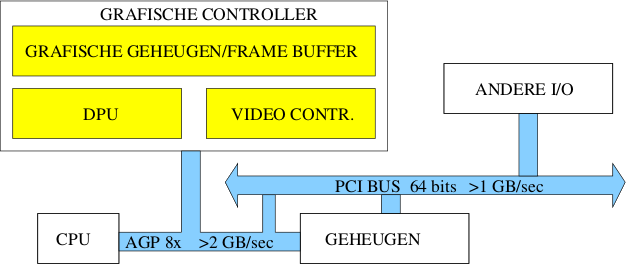
\includegraphics[scale=0.4, angle=0]{plaatjes/agp.png}}
		\end{center}
		
		
		
		In plaats van \verb!scale=x! kan je beter de relatieve afmeting
		\verb!width=\Procent{y}! gebruiken. De waarde $y$ wordt in de
		verslag-mode met uitproberen gevonden, zie figuur~\ref{fig:PDFR}.
		
		\begin{center}
			
			%	\figuur{width=\columnwidth}{plaatjes/2020/eerste oplevermoment/knop.png}{PNGR}{Variabele breedte (png)}
			\subfloat[The net of (c) after firing]{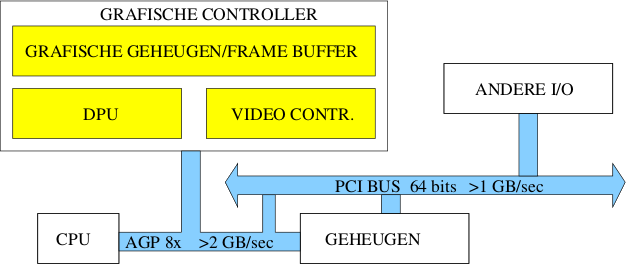
\includegraphics[scale=0.4, angle=0]{plaatjes/agp.png}}
		\end{center}
		
		
		Het afmetingsprobleem is iets gemakkelijker op te lossen met `bitmap
		graphics' van het `jpg-', `gif-' en `png-' formaat omdat de figuren al
		van te voren geschaald kunnen worden als de `bounding box' bij het
		inlezen bekend is. De breedte (\verb!width!) kan als percentage van de
		kolombreedte (\verb!width=\Procent{0 ... 99}!) worden opgegeven zoals
		dat bij figuur~\ref{fig:PNGR} gedaan is. Voor een 100\% waarde neemt
		men \verb!width=\columnwidth! De afmeting wordt automatisch
		aangepast aan de nieuwe kolombreedte.
		
		
		
		\begin{center}
			\begin{tabular}{|>\C p{\Procent{80}}|}
				\hline
				~\\
				Use case\\
				~\\
				Wachten voor de sluis\\
				~\\
				\hline
			\end{tabular}
		\end{center}
		
		
		
		
		\begin{center}
			\begin{tabular}{|>\C p{\Procent{80}}|}
				\hline
				~\\
				Use case\\
				~\\
				Sluis invaren\\
				~\\
				\hline
			\end{tabular}
		\end{center}
		
		
		
		
		
		\begin{center}
			\begin{tabular}{|>\C p{\Procent{80}}|}
				\hline
				~\\
				Use case\\
				~\\
				Sluis uitvaren\\
				~\\
				\hline
			\end{tabular}
		\end{center}
		
		\begin{center}
			
			\subfloat[The net of (c) after firing]{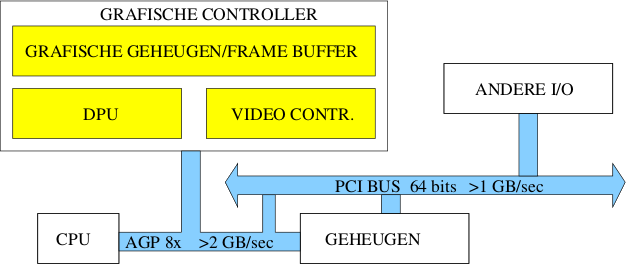
\includegraphics[scale=0.4, angle=0]{plaatjes/agp.png}}
		\end{center}
		
		\begin{center}
			
			\subfloat[The net of (c) after firing]{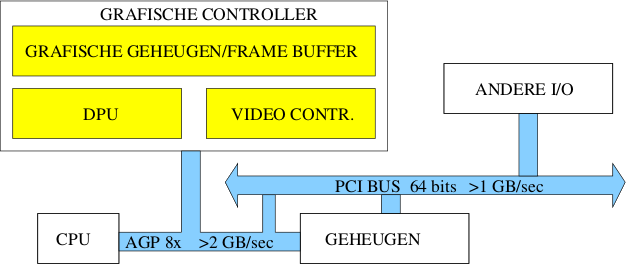
\includegraphics[scale=0.4, angle=0]{plaatjes/agp.png}}
		\end{center}
		
		\begin{center}
			
			\subfloat[The net of (c) after firing]{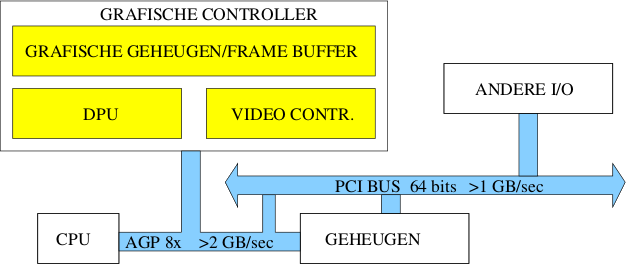
\includegraphics[scale=0.4, angle=0]{plaatjes/agp.png}}
		\end{center}
		
		
		
		
		\begin{center}
			\begin{tabular}{|>\C p{\Procent{80}}|}
				\hline
				~\\
				Use case\\
				~\\
				Meerdere niveaus\\
				~\\
				\hline
			\end{tabular}
		\end{center}
		
		De macro \verb!\PROCENT{0...99}! is nodig voor de macro's \verb!Tabel!
		en \verb!Figuur!. Deze laatste twee macro's maken het mogelijk dat
		tabellen en afbeeldingen in de twocolumn-mode passen met behoud van
		hun originele afmeting en detaillering (zie
		figuur \ref{fig:FIXED}). De parameters van deze macro's komen overeen
		met de parameters van de macro's \verb!tabel! en \verb!figuur!.
		
		
		
		In het algemeen heeft vector-graphics een betere kwaliteit van de
		weergave dan bitmap-graphics.
		
		
		\paragraaf{Bijzondere tekens en afbreekproblemen}
		
		Bijzondere tekens zoals de á, à, ä, é, è, ë, ï, ü, ç \ldots worden
		probleemloos door \LaTeX{} geaccepteerd als normale utf8
		karakters. Voor de uitzonderingen bestaan macro's zoals het
		euro-symbool \euro{} waarvoor de macro \verb!\euro! nodig is. In
		wiskundige formules kan je gebruik maken van de macro \verb!\eurom!.
		
		
		In de two-columnmode zijn regels soms te lang als er gebruik gemaakt
		is van \verb!verb! of \verb!verbatim! of woorden die niet goed worden
		afgebroken. In dat laatste geval kan je in zo'n woord een afbreekpunt
		introduceren met de twee tekens \verb!\-!. Een regel kan gecontroleerd
		afgebroken door van te voren onzichtbare knikpunten te plaatsen met de
		\verb!\Knak! macro. De volgende regel moet in in tegenstelling met de
		twocolumnmode in de verslagmode ongeknakt worden weergegeven:
		
		\begin{Aanpassen}
			\begin{verbatim}
				... aaaaaaa\Knak{}aaaaaaa ...
			\end{verbatim}
		\end{Aanpassen}
		
		
		aaaaaaaaaaaaaaaaaaaaaaaaaaaaaaaaaaaaaaa\Knak{}aaaaaaaaaaaaaaaaaaaaaaaaaaaaaaaaaaaaaaa.
		
		Voor regels waarbij de structuur niet gebroken mag worden, is de
		\verb!\Knak!-methode ongeschikt, bijvoorbeeld bij scripts en
		broncode. Daarentegen zorgt de \verb!Aanpassen!-omgeving ervoor dat in
		de twocolumn-mode de regels met behoud van de originele structuur
		worden weergegeven. Daarvoor wordt een kleinere letterafmeting
		gebruikt (default de \verb!\scriptsize!). Deze omgeving werkt alleen
		met niet al te lange regels. Bij zeer lange regels moet de
		letterafmeting zeer klein worden waardoor de leesbaarheid in het
		gedrang komt. In dat geval moet naar een andere oplossing gezocht
		worden zoals het opnemen van de probleemregels (broncode en scripts)
		in de bijlagen.
		
		\begin{Aanpassen}[\tiny]
			aaaaaaaaaaaaaaaaaaaaaaaaaaaaaaaaaaaaaaaaaaaaaaaaaaaaaaaaaaaaaaaaaaaaaaaaaaaaaa.
		\end{Aanpassen}
		
		Hoewel het gebruik van opsommingen (\verb!\item!), letterlijke citaten
		\verb!quotation! en kaders (\verb!\fbox!) in de twocolumn-mode tot
		problemen kunnen leiden, zijn ze beperkt toegestaan. Bijvoorbeeld voor
		de kaders rond de teksten kan je beter gebruik maken van de
		\verb!tabular!-omgeving (of de \verb!tabel!-omgeving als je geen last
		wil hebben van pagina-overgangen), dan voor de standaard
		\verb!\fbox!-methode. De kolom van deze omkaderde tabel moeten dan wel
		een relatieve afmetingsverhouding de \verb!\columnwidth! krijgen.
		
		\begin{Aanpassen}
			\begin{verbatim}
				\begin{center}
					\begin{tabular}{|>\C p{\Procent{80}}|}
						\hline
						Afbreekproblemen ...
						\hline
					\end{tabular}
				\end{center}
			\end{verbatim}
		\end{Aanpassen}
		
		\begin{center}
			\begin{tabular}{|>\C p{\Procent{80}}|}
				\hline
				~\\
				Afbreek- en andere opmaakproblemen pak je als laatste aan,
				dus bij je definitieve verslag!\\
				~\\
				Tabellen, figuren en listingen in het hoofdverslag tot het
				noodzakelijke beperken.\\
				~\\
				\hline
			\end{tabular}
		\end{center}
		
		
		\paragraaf{Algoritmen en broncode\cite{wikibooks}}
		
		Als je algoritmen met een mooie layout wilt hebben, dan zou je het
		\verb!algorithmic!-pakket kunnen gebruiken. Met dit pakket kan je het
		algoritme op een logische manier opbouwen met pseudotaal. Het bestand
		`verslag.tex' bevat al de pakketten \verb!algorithmic! en
		\verb!listings! die voor dit verslag nodig zijn. Als je zelf packages
		wil toevoegen of verwijderen (afblijven van
		\verb!\usepackage{moduleverslag}!)  dan moet dat in de preambule
		`verslag.tex'.
		
		\begin{Aanpassen}
			\begin{verbatim}
				\usepackage{algorithmic}
			\end{verbatim}
		\end{Aanpassen}
		
		Een algoritme moet je maken binnen een algorithmic-omgeving, een
		voorbeeld:
		
		\begin{Aanpassen}[\small]
			\begin{algorithmic}
				\IF {$i\geq maxval$} 
				\STATE $i\gets 0$
				\ELSE
				\IF {$i+k\leq maxval$}
				\STATE $i\gets i+k$
				\ENDIF
				\ENDIF 
			\end{algorithmic}
		\end{Aanpassen}
		
		
		Broncode kan je in een \verb!verbatim!-omgeving opnemen. De
		broncoderegels zien er net zo uit zoals je ze ingetypt hebt.  Het
		\verb!listings!-pakket is geavanceerder dan de
		\verb!verbatim!-omgeving.
		
		\begin{Aanpassen}
			\begin{verbatim}
				\usepackage{listings}
			\end{verbatim}
		\end{Aanpassen}
		
		Merk even op dat alle commando's van het \verb!listings!-pakket
		beginnen met \verb!lst!, dit conform de lppl-licentie.
		
		De broncode zelf zet je in een \verb!listings!-omgeving, net zoals bij
		de \verb!verbatim!-omgeving, om broncode te zetten gebruik je het
		\verb!\lstinline!-commando op dezelfde manier als het
		\verb!\verb!-commando. Je kunt ook broncode van een extern document laden met het commando:
		
		\begin{Aanpassen}
			\begin{verbatim}
				\lstinputlisting{pathname}
			\end{verbatim}
		\end{Aanpassen}
		
		Het argument `pathname' is de relatieve of absolute locatie van het
		bronbestand, de map(pen) gecombineerd met de bestandsnaam. Als je
		broncode van een bronbestand laadt, ben je zeker dat de broncode in je
		\LaTeX{}-document altijd actueel is en hou je het \LaTeX{}-document
		overzichtelijk. Als de broncode niet in dezelfde map of een submap van
		het \LaTeX{}-document staat of je gebruikt absolute `pathnames', dan
		is het mogelijk dat het verslag niet op andere computers gecompileerd
		kan worden. Bij het inleveren van je afstudeerverslag in
		\LaTeX{}-formaat zal je hiermee rekening moeten houden.
		
		
		Alle opties in het \verb!listings!-pakket hebben eenzelfde structuur
		\verb!sleutel=waarde!. Als je alleen 'Java' gebruikt hebt, dan kan je
		deze taal voor je volledig document na de regel
		\verb!\usepackage{listings}! in preambule `verslag.tex' definiëren met
		\verb!\lstset{language=java}!
		
		\lstset{language=java}
		
		\begin{Aanpassen}
			\begin{lstlisting}
				public class HelloWorld {
					public static void main(String[] args) {
						System.out.println("Hello, world!");
					}
				}
			\end{lstlisting}
		\end{Aanpassen}
		
		
		De sleutel is hier dus \verb!language! en de waarde die je aan de
		sleutel geeft is \verb!java!. Alles wat je als opties binnen de
		\verb!\lstset!-macro zet kan je per \verb!listings!-omgeving apart
		definiëren. Bijvoorbeeld html-broncode met
		\verb!\begin{lstlisting}[language=html]!:
			
			\begin{Aanpassen}
				\begin{lstlisting}[language=html]
					<html>
					<head>
					<title>Hello</title>
					</head>
					<body>Hello</body>
					</html>
				\end{lstlisting}
			\end{Aanpassen}
			
			\subsection{Conclusie}
			
			
			
			Om een goed verhaal op te stellen, moet vooraf aan enkele voorwaarden
			worden voldaan. De eerste voorwaarde is de geschiktheid van het
			afstudeerproject. Als een afstudeerproject niet tot keuzes leidt, kan
			men zich afvragen of dat wel een echte afstudeeropdracht is. Een
			afstudeerproject zonder onderzoeksaspecten is ook verdacht. Daarnaast
			moet een afstudeerproject passen in het profiel van een opleiding om
			beoordeelbaar te zijn. De andere voorwaarde voor goed een verhaal is
			de registratie van werkzaamheden tijdens het a
			worden voldaan. De eerste voorwaarde is de geschiktheid van het
			afstudeerproject. Als een afstudeerproject niet tot keuzes leidt, kan
			men zich afvragen of dat wel een echte afstudeeropdracht is. Een
			afstudeerproject zonder onderzoeksaspecten is ook verdacht. Daarnaast
			moet een afstudeerproject passen in het profiel van een opleiding om
			beoordeelbaar te zijn. De andere voorwaarde voor goed een verhaal is
			de registratie van werkzaamheden tijdens het a
			
			
			Subheadings reflect the content and organization of the different parts of the main text. Each paragraph may cover one idea, characteristic or topic. Don’t refer only one study in each paragraph.Wherever required, link the research findings to the research problem described in the introduction. Three tenses (simple present, simple past and present perfect) are frequently used. Length of this section is about 70% to 90% of main text.
			
			
			22)   Present your results in logical sequence  in the text,tables and illustrations.  Do not repeat in the text all the data, in the tables or illustrations.
			23)   Emphasize or summarize important observations.Results  section should contain only  actuals, and no opinions.
			24)   All  the  patients  included  in  the  study  should  be accounted for. There should not be any hesitation in reporting any negative or unexpected result.
			
			
			
			\begin{figure}[!ht]
				\centering
				\begin{floatrow}
					\ffigbox[\FBwidth]{\caption{Dummy figure}\label{fig:dummy-1}}{%
						\rule{1.6in}{0.9in}   % Just a dummy. Replace with your figure.
					}
					\ffigbox[\FBwidth]{\caption{Dummy figure}\label{fig:dummy-2}}{%
						\rule{1.6in}{0.9in}   % Just a dummy. Replace with your figure.
					}
					
					\ffigbox[\FBwidth]{\caption{Dummy figure}\label{fig:dummy-1}}{%
						\rule{1.6in}{0.9in}   % Just a dummy. Replace with your figure.
					}
					\ffigbox[\FBwidth]{\caption{Dummy figure}\label{fig:dummy-2}}{%
						\rule{1.6in}{0.9in}   % Just a dummy. Replace with your figure.
					}
				\end{floatrow}
			\end{figure}
			
			
			\begin{figure}[!tbp]
				\centering
				\subfloat[Flower one.]{\includegraphics[width=0.4\textwidth]{flower1.jpg}\label{fig:f1}}
				\hfill
				\subfloat[Flower two.]{\includegraphics[width=0.4\textwidth]{flower2.jpg}\label{fig:f2}}
				\caption{My flowers.}
				\subfloat[Flower one.]{\includegraphics[width=0.4\textwidth]{flower1.jpg}\label{fig:f1}}
				\hfill
				\subfloat[Flower two.]{\includegraphics[width=0.4\textwidth]{flower2.jpg}\label{fig:f2}}
				\caption{My flowers.}
			\end{figure}
			
			
			
			\section{testresultaten}
			Om een goed verhaal op te stellen, moet vooraf aan enkele voorwaarden
			worden voldaan. De eerste voorwaarde is de geschiktheid van het
			afstudeerproject. Als een afstudeerproject niet tot keuzes leidt, kan
			men zich afvragen of dat wel een echte afstudeeropdracht is. Een
			afstudeerproject zonder onderzoeksaspecten is ook verdacht. Daarnaast
			moet een afstudeerproject passen in het profiel van een opleiding om
			beoordeelbaar te zijn. De andere voorwaarde voor goed een verhaal is
			de registratie van werkzaamheden tijdens het a
			
			
			\begin{tabular}{|l|l {2cm} |l|l|l|l|l|l|l|l|} \hline
				\multicolumn{10}{|l|}{REQ traceabilitymatrix}                                                               \\ \hline
				\multicolumn{4}{|l|}{project name}   &\multicolumn{6}{|l|}{Created designed by}                           \\ \hline
				\multicolumn{4}{|l|}{release no}   &\multicolumn{6}{|l|}{Created on}                           \\ \hline
				\multicolumn{4}{|l|}{version}   &\multicolumn{6}{|l|}{Reviewed on}                           \\ \hline
				\multicolumn{4}{|l|}{Test title}   &\multicolumn{6}{|l|}{Reviewed by}                           \\ \hline
				\multicolumn{4}{|l|}{Description}   &\multicolumn{6}{|l|}{ }                           \\ \hline 		
				\multicolumn{10}{|l|}{ }   																\\ \hline
				\multicolumn{10}{|l|}{Pre condition}                                                               \\ \hline
				\multicolumn{10}{|l|}{Dependencies}                                                               \\ \hline
				\multicolumn{10}{|l|}{ }   															\\ \hline
				\multicolumn{2}{|l|}{REQ ID} & description & Status &Designdoc &codemodule&testaseID &T.case Name & manual& testedon \\ \hline
				\multicolumn{2}{|l|}{REQ ID} &  \thead{ Als  \\gebruiker \\	wil ik  \\een  \\ 	ssid  \\invoeren   }
				& Status &Designdoc &codemodule&testaseID &T.case Name & manual& testedon \\ \hline
				\multicolumn{2}{|l|}{REQ ID} &  \thead{ Als  \\gebruiker \\	wil ik  \\een  \\ 	ssid  \\invoeren   }
				& Status &Designdoc &codemodule&testaseID &T.case Name & manual& testedon \\ \hline
				\multicolumn{2}{|l|}{REQ ID} &  \thead{ Als  \\gebruiker \\	wil ik  \\een  \\ 	ssid  \\invoeren   }
				& Status &Designdoc &codemodule&testaseID &T.case Name & manual& testedon \\ \hline
				\multicolumn{2}{|l|}{REQ ID} &  \thead{ Als  \\gebruiker \\	wil ik  \\een  \\ 	ssid  \\invoeren   }
				& Status &Designdoc &codemodule&testaseID &T.case Name & manual& testedon \\ \hline
			\end{tabular}
			
			
			
			
			
			
			
			\subsection{Testcases}		
			
			Om een goed verhaal op te stellen, moet vooraf aan enkele voorwaarden
			worden voldaan. De eerste voorwaarde is de geschiktheid van het
			afstudeerproject. Als een afstudeerproject niet tot keuzes leidt, kan
			men zich afvragen of dat wel een echte afstudeeropdracht is. Een
			afstudeerproject zonder onderzoeksaspecten is ook verdacht. Daarnaast
			moet een afstudeerproject passen in het profiel van een opleiding om
			beoordeelbaar te zijn. De andere voorwaarde voor goed een verhaal is
			de registratie van werkzaamheden tijdens het a
			
			
			
			\begin{tabular}{|l|l|l|l|l|l|l|} \hline
				\multicolumn{7}{|l|}{project name}                                                               \\ \hline
				\multicolumn{4}{|l|}{Test case ID}   &\multicolumn{3}{|l|}{Test designed by}                           \\ \hline
				\multicolumn{4}{|l|}{test priority (low/medium/high)}   &\multicolumn{3}{|l|}{Test design date}                           \\ \hline
				\multicolumn{4}{|l|}{Module name}   &\multicolumn{3}{|l|}{Test executed by}                           \\ \hline
				\multicolumn{4}{|l|}{Test title}   &\multicolumn{3}{|l|}{Test execution date}                           \\ \hline
				\multicolumn{4}{|l|}{Description}   &\multicolumn{3}{|l|}{ }                           \\ \hline 		
				\multicolumn{7}{|l|}{ }   																\\ \hline
				\multicolumn{7}{|l|}{Pre condition}                                                               \\ \hline
				\multicolumn{7}{|l|}{Dependencies}                                                               \\ \hline
				\multicolumn{7}{|l|}{ }   															\\ \hline
				Step  &  Test steps & Test data & expected result &Acual result &Streee (pass or fail)&notes  \\ \hline
				
			\end{tabular}
			
			
			
			
			
			
			
			\subsection{Reparaties}
			
			\subsection{Resulaat annalyse}
			
			\lipsum[2-4]
			\begin{figure}[t]
				\centering
				\subfloat[Net is not enabled because multiplicity of read arc $<2$] {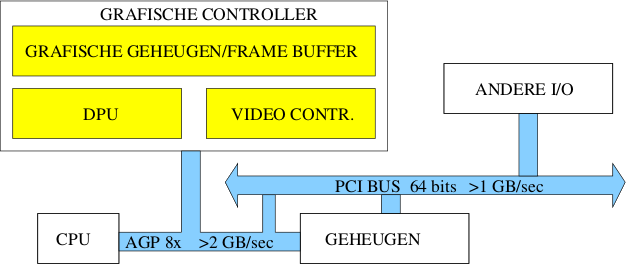
\includegraphics[scale=0.4, angle=0]{plaatjes/agp.png}}\hfil
				\subfloat[Net is not enabled C $>1$] {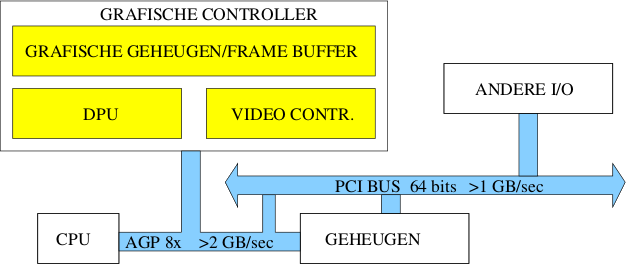
\includegraphics[scale=0.4, angle=0]{plaatjes/agp.png}}
				
				\subfloat[The net is enabled]{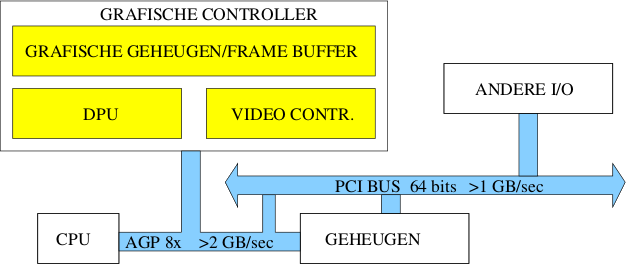
\includegraphics[scale=0.4, angle=0]{plaatjes/agp.png}}\hfil
				\subfloat[The net of (c) after firing]{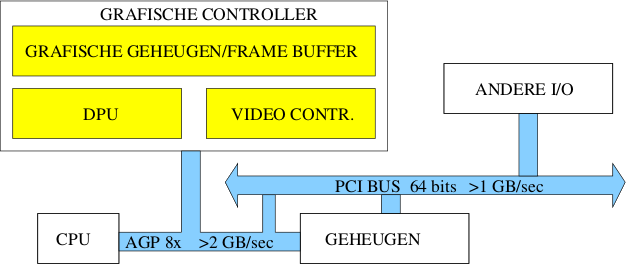
\includegraphics[scale=0.4, angle=0]{plaatjes/agp.png}}
				\caption{}
				
				
				\label{fig: 2.2}
			\end{figure}
			
			
			\subsection{Reparaties}
			
			\subsection{Resulaat annalyse}
			
			\lipsum[2-4]
			\begin{figure}[t]
				\centering
				\subfloat[Net is not enabled because multiplicity of read arc $<2$] {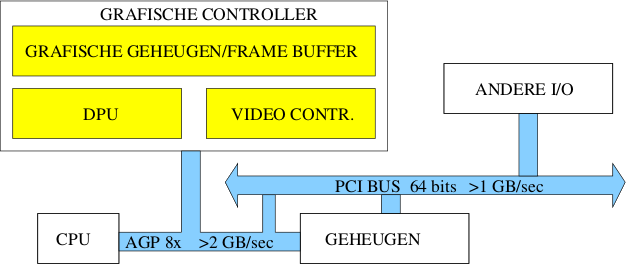
\includegraphics[scale=0.4, angle=0]{plaatjes/agp.png}}\hfil
				\subfloat[Net is not enabled C $>1$] {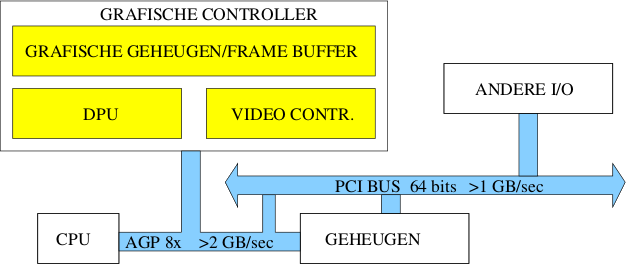
\includegraphics[scale=0.4, angle=0]{plaatjes/agp.png}}
				
				\subfloat[The net is enabled]{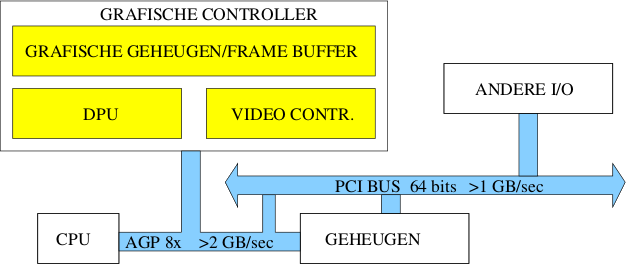
\includegraphics[scale=0.4, angle=0]{plaatjes/agp.png}}\hfil
				\subfloat[The net of (c) after firing]{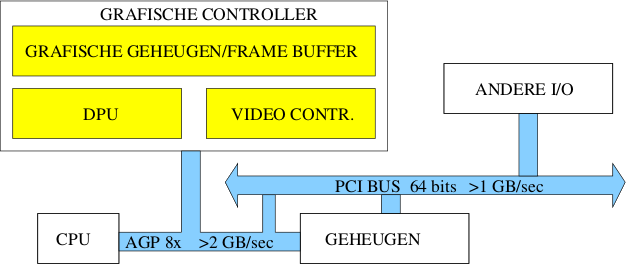
\includegraphics[scale=0.4, angle=0]{plaatjes/agp.png}}
				\caption{}
				
				
				\label{fig: 2.2}
			\end{figure}
			
			%%%%%%%%%%%%%%%%%%%%%%%%%%%%%%%%%%%%%%%%%%%%%%%%%%%%%%%%%%%%%%
